\section{Раработка программного обеспечения}

\subsection{Разработка серверной части}

Структура приложения, написанного на фреймворке Django представляет собой набор отдельных приложений, выполняющих отдельные функции.
Каждое приложение вклбчает в себя:
\begin{itemize}
    \item models.py - файл, содержащий представление моделей базы данных;
    \item migrations/ - папка, хранящая миграции моделей;
    \item serialzers.py - файл, содержащий представления входных/выходных данных сервера;
    \item views.py - файл, содержащий контроллеры, обрабатывающие запросы;
    \item utils.py - файл, содержащий вспомогательные функции приложения, например сервисы обращения к третьим приложения;
    \item tasks.py - файл, содержищий асинхронные-задачи данного приложения, которые взаимодействуют с моделями это приложения, либо логически относятся к нему;
    \item tests.py - файл, содержащий тесты к контроллерам;
    \item factories.py - файл, содержащий фабрики для генерации данных для тестов;
    \item permissions.py - файл, содержащий пользовательские разрешения для запросов;
    \item signals.py - файл, содержащий сигналы для моделей БД;
    \item admin.py - файл, содержаший модели представления и модификации сайта администратора;
    \item urls.py - файл, содержищий связи между контроллерами и url-адресами.
\end{itemize}

Хоть Django фреймворк и предоставляет готовую структуру для написания веб-приложения, однако в каждом проекте присутствуют утилиты, нужные в независимости от приложения.
К таким утилитам относятся работы со структурами данных, работа с изображениями и интернализацией, миксины для контроллеров, сериализаторов либо тестов и тд.
Для таких утилит на уровне приложений была создана отдельная папка <<utils>>, содержащая модули python, разбитые по категориям:
\begin{itemize}
    \item strings.py - файл, содержащий утилиты для работы со строками;
    \item tests.py - папка, содержащий утилиты для работы с тестами;
    \item constants.py - файл, содержащий константы приложения;
    \item mixins.py - файл, содержащий миксины для сериализаторов и контроллеров;
    \item images.py - файл, содержащий утилиты для работы с изображениями;
    \item i18l.py - файл, содержащий утилиты для рабоыт с интернализацией;
    \item models.py - файл, содержащий утилиты для рабоыт с моделями.
\end{itemize}

Для предоставления возможности масштабирования системы была выбрана плоская структура конечных точек HTTP[19].
Данная структура характеризуется большим объемом мелких конечных точек, отвечающих за отдельные сущность.
Одновременно минусом и плюсом данной структуры является, как оговаривалось раньше, возможность получения конкретных объектов базы данных по средством отдельных конечных точек.
Таким образом, например, для получения всех данных о пользователе, клиент должен будеть послать несколько запросов к серверу.
Данная архитектура увеличивает количество запросов к серверу, однако сложно представить, что на одной странице клиента будут отображены все данные о пользователе.
И при нескольких конечных точках возможно, при ее необходимости, закгрузка данных в фоне.

На основании выбора плоской архитектуры к организации программного интерфейса к серверной части приложения были реализованы приложения: Auth, Users, Goods, Payments, Orders, Addresses.
Итоговая структура проекта представлена на рисунке 4.1.

\begin{figure}[h!]
    \begin{subfigure}[b]{0.3\textwidth}
    \centering
    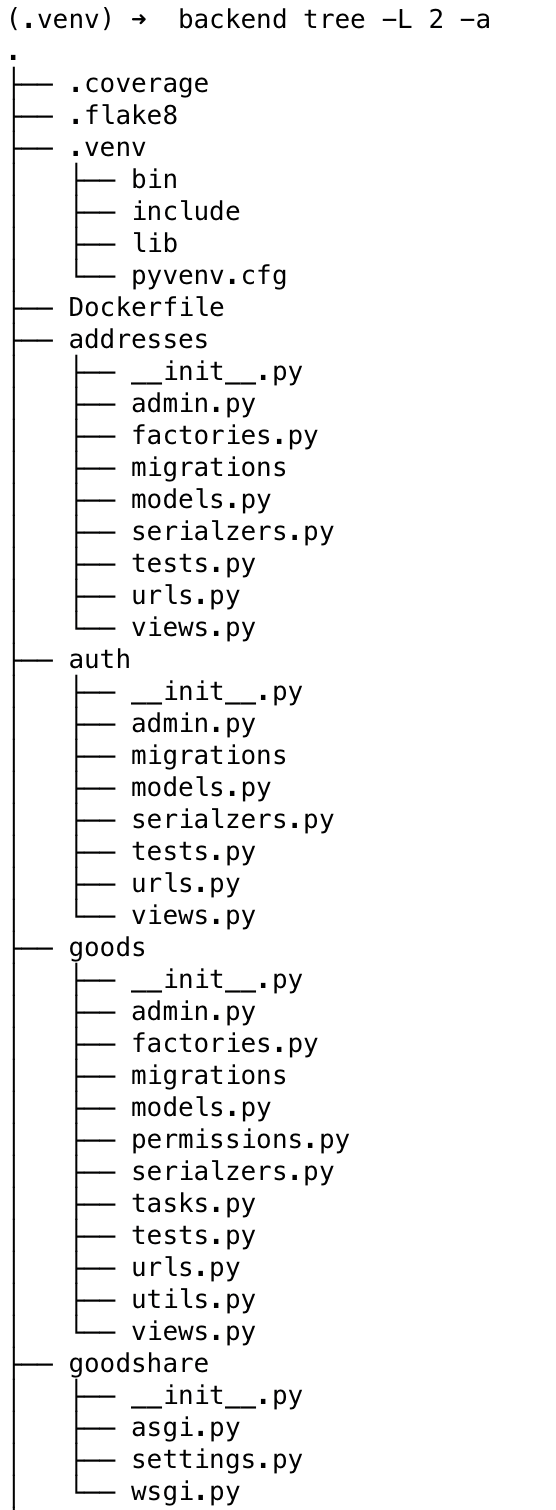
\includegraphics[scale=0.8]{structure_1.png}
    \caption{}
    \end{subfigure}
    \begin{subfigure}[b]{0.3\textwidth}
    \centering
    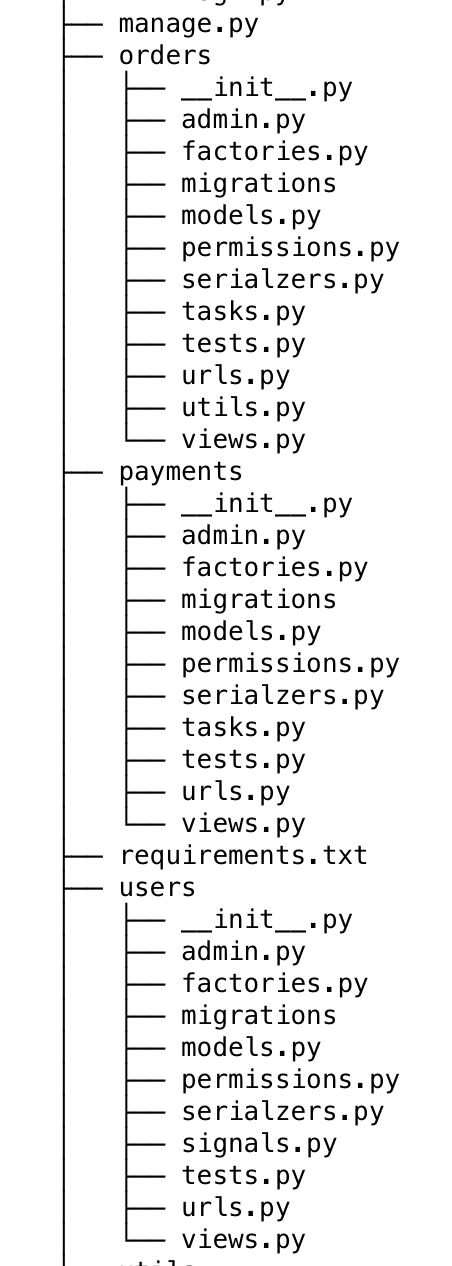
\includegraphics[scale=0.8]{structure_2.png}
    \caption{}
    \end{subfigure}
    \begin{subfigure}[b]{0.3\textwidth}
    \centering
    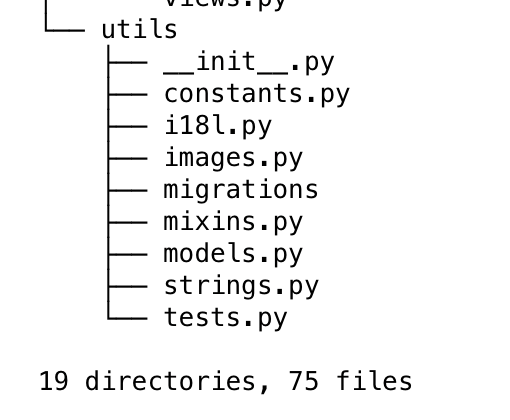
\includegraphics[scale=0.8]{structure_3.png}
    \caption{}
    \end{subfigure}
    \caption{ Структура серверной части приложения }
    \label{fig:fire_alarms}
\end{figure}


\begin{longtable}{ | l | p{6cm} | }
    \hline
    Название приложения & Выполняющие функции \\ \hline
    Auth & Отвечает за процесс авторизации пользователя в системе \\ \hline
    Users & Отвечает за манипуляции с пользовательскими данными \\ \hline
    Goods & Отвечает за доступ к товарам и взаимодействия с ними \\ \hline
    Payments & Хранения сохранненых данных для оплаты пользователя\\ \hline
    Orders & Хранения и соверщение заказов пользователя \\ \hline
    Addresses & Хранения адресов оплаты пользователя \\ \hline
\end{longtable}



\subsubsection{Программный интерфейс серверной части}
На основании функциональных требований в каждом приложении были реализованы API конечных точек HTTP-запросов.

Приложение Auth, базовый url адрес конечных точек <</auth>>.

\begin{longtable}{ | p{3cm} | p{4cm} | p{3cm} | p{3cm} | }
    \hline
    url-адрес запроса / метод запроса & входные данные & выходные данные  & описание \\ \hline
   /verify POST  & phone - номер телефона, token - токен, выданные firebase, после вводна OTP кода & token - токен авторизации пользователя для осузествления запросов к серверу & С помощью данного запроса пользователь может авторизироваться в приложении с помощью токена \\ \hline
\end{longtable}

Приложение Users, базовый url адрес конечных точек <</users>>.

\begin{tabular}{ | p{3cm} | p{4cm} | p{3cm} | p{3cm} | }
    \hline
    url-адрес запроса / метод запроса & входные данные & выходные данные  & описание \\ \hline
    / POST & name - ФИО пользователя, photo - фото пользователя & созданная модель пользователя & создание пользователя в системе \\ \hline
    / PUT & name - ФИО пользователя, photo - фото пользователя, email - электронная почта пользователя & обновленная модель пользователя & обновление данных пользователя \\ \hline
    /ID/review POST & text - текст отзыва, mark - оценка пользователя & & создание отзыва о пользователе \\ \hline
    / GET & & получение информации о пользователе \\ \hline
\end{tabular}

Приложение Addresses, базовый url адрес конечных точек <</addresses>>.

\begin{longtable}{ | p{3cm} | p{4cm} | p{3cm} | p{3cm} | }
    \hline
    url-адрес запроса / метод запроса & входные данные & выходные данные  & описание \\ \hline
    / POST & city - город получателя, street - улица получателя, building - номер здания получателя, appartament - номер квартиры получателя & созданная модель адреса & создания адреса доставки пользователя \\ \hline
    /ID PUT & city - город получателя, street - улица получателя, building - номер здания получателя, appartament - номер квартиры получателя & обновленная модель адреса & обновление адреса доставки пользователя \\ \hline
    /ID DELETE & & & удаление адреса доставки пользователя \\ \hline
    / GET & & & получение всех сохраенных записей адресов \\ \hline
\end{longtable}

Приложение Payments, базовый url адрес конечных точек <</payments>>.

\begin{longtable}{ | p{3cm} | p{4cm} | p{3cm} | p{3cm} | }
    \hline
    url-адрес запроса / метод запроса & входные данные & выходные данные  & описание \\ \hline
    / POST & card\_number - номер карты пользователя, cvv\_code - cvv-код карты, date\_expire - срок годности карты, cardholder\_name - имя держателя карты & созданная модель оплаты & создание модели оплаты пользователя \\ \hline
    /ID PUT & card\_number - номер карты пользователя, cvv\_code - cvv-код карты, date\_expire - срок годности карты, cardholder\_name - имя держателя карты & обновленная модель оплаты & обновление модели оплаты пользователя \\ \hline
    /ID DELETE & & & удаление модели оплаты \\ \hline
    / GET & & получение всех сохраенных записей оплат \\ \hline
\end{longtable}

Приложение Goods, базовый url адрес конечных точек <</goods>>.

\begin{longtable}{ | p{3cm} | p{4cm} | p{3cm} | p{3cm} | }
    \hline
    url-адрес запроса / метод запроса & входные данные & выходные данные  & описание \\ \hline
    /add POST & name - название товара, condition - состояние товара, description - описание товара, can\_be\_purchased - возможность выкупа товара, price\_per\_hour - цена аренды товара за час, price\_per\_day - цена аренды товара за сутки, own\_deliver - возможность доставки товара арендадателем & созданная модель товара & создания товара \\ \hline
    /ID PUT & name - название товара, condition - состояние товара, description - описание товара, can\_be\_purchased - возможность выкупа товара, price\_per\_hour - цена аренды товара за час, price\_per\_day - цена аренды товара за сутки, own\_deliver - возможность доставки товара арендадателем & обновленная модель товара & обновление информации о товаре \\ \hline
    /ID DELETE & & & удаление товара \\ \hline
    /ID/add-to-basket PUT &  & & добавление товара в корзину \\ \hline
    /ID/remove-from-basket PUT & & & удаление товара из корзины \\ \hline
    /?page=PAGE GET & PAGE - страница поисков & список моделей товаров & получить все товары \\ \hline
    /?page=PAGE \&XX=YY GET & PAGE - страница поисков, XX=элемент фильтрации, YY -  значение XX фильтра & список моделей товаров & получить все товары \\ \hline
\end{longtable}

Приложение Orders, базовый url адрес конечных точек <</orders>>.

\begin{longtable}{ | p{3cm} | p{4cm} | p{3cm} | p{3cm} | }
    \hline
    / POST & start\_use\_date - дата начала пользования, end\_use\_date - дата окончания пользования, payment - выбор оплаты, address - выбор адреса доставки & модель заказа & создание заказа \\ \hline
    /ID/pay PUT & & & оплата товара; \\ \hline
    / GET & & список моделей заказов & получение списка заказов. \\ \hline
\end{longtable}

\subsubsection{Построение диаграммы компонентов серверной части}
Описать структуру бека, взаимодействия с БД и Firebase
Добавить приложение с диаграммой

\subsection{Разработка клиентской части}

Как было описано в разделе про проектирование клиентской части, в среде React приложений нет четко выработанной структуры приложений.
Однако основываясь на практиках написания React приложений была реализованна структура приложения, представленная на рисунке 4.2.

Глобальное состояние приложения была разделено на несколько редьюсеров:
\begin{itemize}
    \item appReducer - котнролирует глобальное состояние приложение, а именно контроль отображения загрузчиков в приложении;
    \item authReducer - контролирует изменение и процесс аунтентификации пользователя;
    \item basketReducer - контролирует состояние корзины пользователя;
    \item checkoutReducer - контролирует процесс покупки товара;
    \item filterReducer - отвечает за фильтрацию товаров на экране поиска товаров;
    \item productReducer - отвечает за создание и изменения пользовательских продуктов;
    \item profileReducer - отвечает за состяние пользовательских данных;
    \item orderReducer - отвечает за состояние пользовательских заказов;
\end{itemize}

Соответственно каждому редьюсеру были созданы саги, экшены и константы, которые провоцируют приложению на осуществление запросов на сервер либо изменение состояния.

Компоненты приложения расположены в директориях <<components>> и <<views>> таким образом, что в директории <<components>> расположены глупые компоненты, представляющие репрезентационные компоненты.
А в дирректории <<views>> расположены как экраны приложения, так и компоненты-контейнеры.

\begin{figure}[h!]
    \begin{subfigure}[b]{0.45\textwidth}
    \centering
    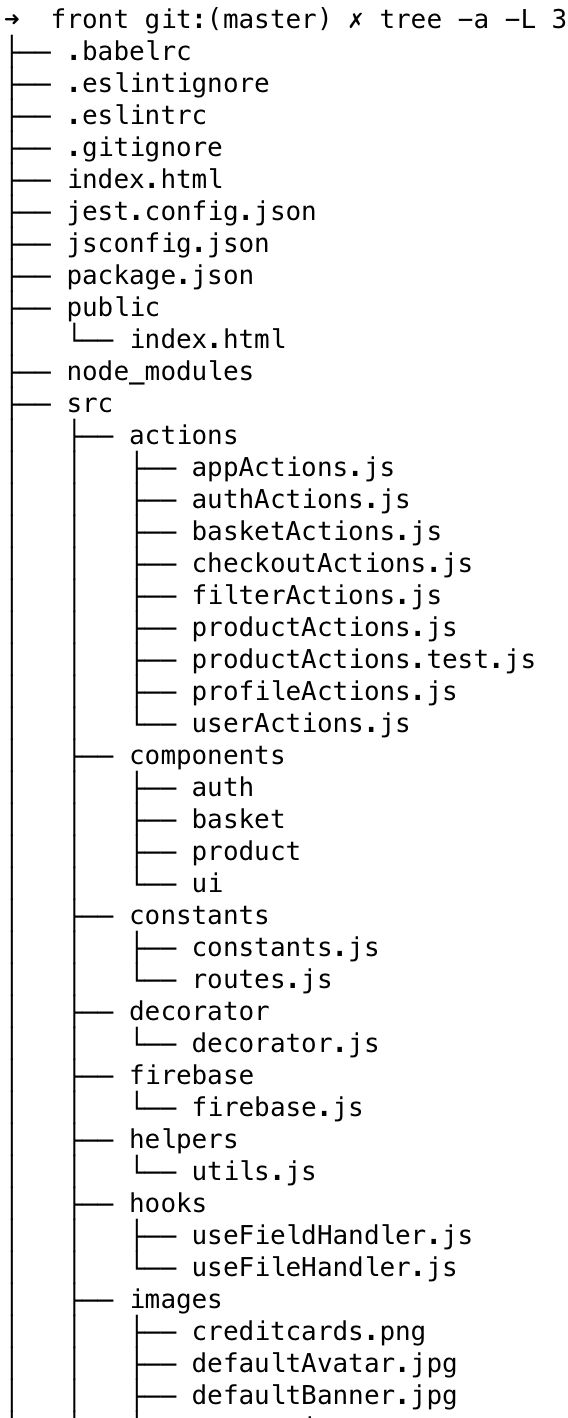
\includegraphics[scale=0.8]{front_structure_1.png}
    \caption{}
    \end{subfigure}
    \begin{subfigure}[b]{0.3\textwidth}
    \centering
    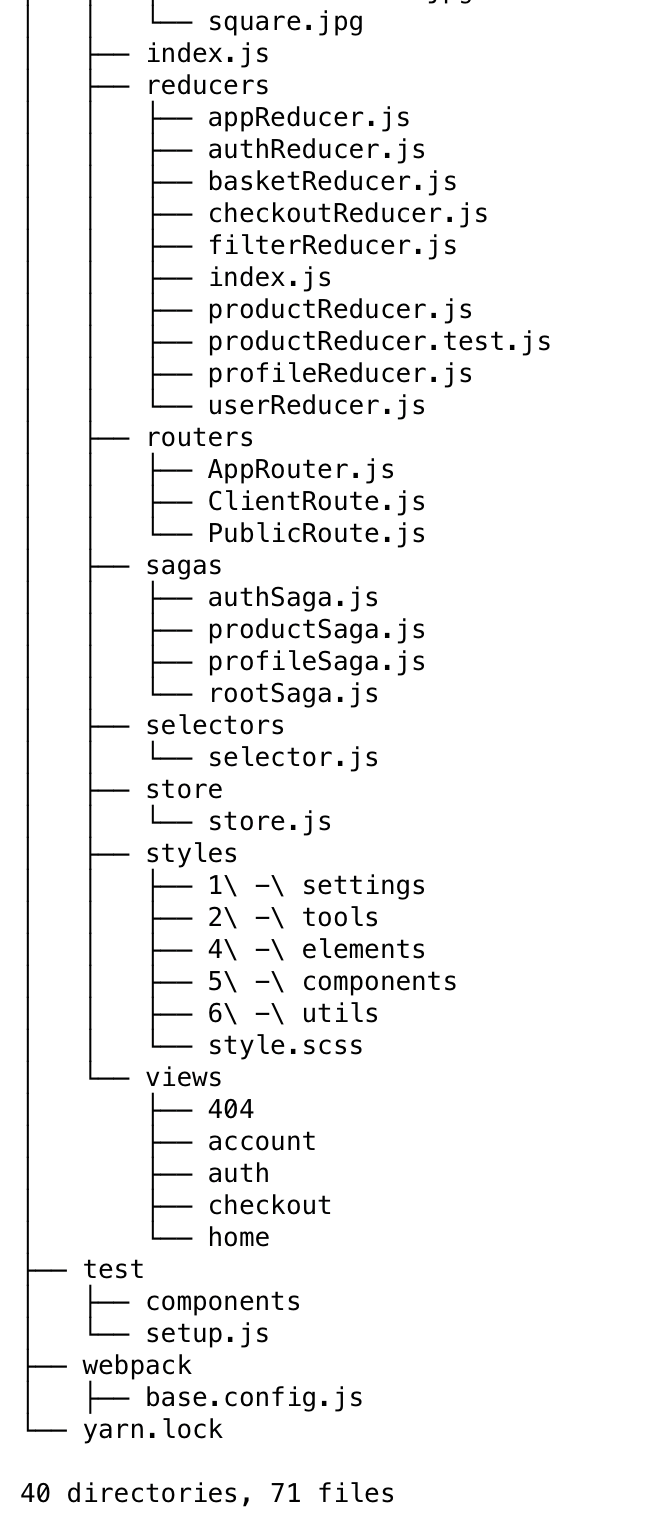
\includegraphics[scale=0.8]{front_structure_2.png}
    \caption{}
    \end{subfigure}
    \caption{ Структура клиентской части приложения }
\end{figure}

В приложении B можно ознакомиться со скриншота веб-приложения.
